\documentclass[a4paper, 14pt]{article}
\usepackage{fontspec, extsizes, geometry, setspace, titlesec, fancyhdr, graphicx, float, setspace, caption, csquotes, color, listings, booktabs}
\newcommand{\bigcell}[2]{\begin{tabular}{@{}#1@{}}#2\end{tabular}}
\usepackage[russian, english, ukrainian]{babel}
\usepackage[dotinlabels]{titletoc}
\bibliographystyle{gost-numeric}
\usepackage[backend=biber, bibstyle=gost-numeric]{biblatex}
\addbibresource{paper.bib}
\setmainfont[Ligatures=TeX]{Times New Roman}
\geometry{a4paper,total={170mm,257mm},left=2cm,top=2cm,bottom=2cm,right=2cm}
\def\changemargin#1#2{\list{}{\rightmargin#2\leftmargin#1}\item[]}\let\endchangemargin=\endlist % удобная команда
\makeatletter\newcommand\Dotfill{\leavevmode\leaders\hb@xt@0.65em{\hss.\hss}\hfill}\makeatother % удобная команда
\let\stdsection\section\renewcommand\section{\newpage\stdsection} % Новая секция -> новая страница
\addto\captionsenglish{\renewcommand{\figurename}{Рис.}} % Подпись картинок
\titleformat{\section}[display]{\filcenter}{\bfseries{РОЗДІЛ \thesection.}}{0pt}{\bfseries\MakeUppercase} % Изменение заголовка всех разделов
\renewcommand{\thesubsection}{\arabic{section}.\arabic{subsection}} % Чиним номер подраздела
\titleformat{\subsection}{\filcenter}{\bfseries \thesubsection. }{0pt}{\bfseries}{} %чиним название подраздела 
\captionsetup{labelsep=period} % "Рис. 1." вместо "Рис. 1:"
\fancyhf{}\renewcommand{\headrulewidth}{0pt}\newcommand{\changefont}{\fontsize{14}{14}\selectfont}\fancyhead[R]{\changefont \thepage}\fancypagestyle{plain}{\fancyhf{}\fancyhead[R]{\changefont \thepage}\renewcommand{\headrulewidth}{0pt}\renewcommand{\footrulewidth}{0pt}}\pagestyle{fancy} %номер страницы справа сверху на всех страничках [это ужас]
\linespread{1.25} %#1
\renewcommand{\contentsname}{ЗМІСТ} %изменяем название странички с содержанием
\def\numberline#1{#1. } % Фикс чтобы названия не налезали друг на друга в содержании
\titlecontents{section}[0pt]{\normalfont}{РОЗДІЛ \thecontentslabel. }{}{\Dotfill \contentspage} % точки в содержании
\titlecontents{subsection}[0pt]{\normalfont}{\thecontentslabel. }{}{\Dotfill \contentspage} % точки в содержании
\titlecontents{subsubsection}[2.25em]{\normalfont}{\thecontentslabel. }{}{\Dotfill \contentspage} % точки в содержании
\newcommand{\RNum}[1]{\uppercase\expandafter{\romannumeral #1\relax}}
\definecolor{dkgreen}{rgb}{0,0.6,0}
\definecolor{gray}{rgb}{0.5,0.5,0.5}
\definecolor{mauve}{rgb}{0.58,0,0.82}
\graphicspath{{./images/}}
\lstset{frame=tb, language=Java,  aboveskip=3mm,  belowskip=3mm,  showstringspaces=false,  columns=flexible,  basicstyle={\small\ttfamily},  numbers=none,  numberstyle=\tiny\color{gray},  keywordstyle=\color{blue},  commentstyle=\color{dkgreen},  stringstyle=\color{mauve},  breaklines=true,  breakatwhitespace=true, tabsize=2
}
\lstset{moredelim=[is][\textit]{[*}{*]}}
\counterwithin{figure}{section}
\counterwithin{table}{section}
\begin{document}
% Титулка
\thispagestyle{empty}
\begin{spacing}{1}
\begin{center}
Міністерство освіти і науки України\\
Департамент науки і освіти Харківської облдержадміністрації\\
Харківське територіальне відділення МАН України\\
\end{center}\par\null\par
\begin{changemargin}{10cm}{0cm}
Відділення: комп'ютерних наук\\
Секція: комп'ютерні системи та мережі
\end{changemargin}\par\null\par
\begin{center}
МЕТОД ПОШУКУ ТА УСУНЕННЯ ПОВТОРЮВАНИХ
ЧАСТИН У ПОЧАТКОВОМУ КОДІ ПРОГРАМНОГО ЗАБЕЗПЕЧЕННЯ
\end{center}\par\null\par\null
\begin{changemargin}{10cm}{0cm}
Роботу виконав:\\ 
Човпан Ігор Сергійович,\\
учень 11 класу Харківського\\
Навчально-виховного комплексу\\
№45 «Академічна гімназія»\\
Харківської міської ради\\
Харківської області
\end{changemargin}\par
\begin{changemargin}{10cm}{0cm}
Науковий керівник:\\
Руккас Кирило Маркович,\\
професор кафедри теоретичної та\\
прикладної інформатики\\
механіко-математичного\\
факультету Харківського\\
національного університету\\
ім. В.Н. Каразіна, доктор\\
технічних наук, доцент\\
\vspace*{\fill}\end{changemargin}
\begin{center}
Харків -- 2020
\end{center}\end{spacing}

% Тези
\section*{Т\lowercase{ези}}
...
\newpage
\tableofcontents %генерация содержания
\newpage
\section*{\textbf{ВСТУП}}
\addcontentsline{toc}{section}{ВСТУП} %добавляем страницу ВСТУП в содержание
Серед розробників програмного забезпечення практика копіювання та вставки коду є досить поширеною. Не дивлячись на те, що це може бути корисним та зручним навиком у короткостроковій перспективі, подібна практика призводить до катастрофічних наслідків при обслуговуванні програмного забезпечення. \\ Так, наприклад, будь яке удосконалення чи усунення помилки потрібно буде робити для кожної копії, що робиться далеко не завжди. Через це істотно збільшується кількість потенційних вразливостей та помилок у коді, на підтримку програмного забезпечення великих розмірів потрібно значно більше ресурсів. \\
Досліди показують, що доволі велику частину від початкового коду проекту займають копії (у середньому 5-10\% \cite{Baxter98}). \\
Через це, пошук та усунення повторюваних частин у початковому коді є важливою задачею. \\
Існує досить багато методів пошуку копій, але в кожного є свої недоліки. Наприклад, у методах, використовуючих абстрактне синтаксичне дерево, головною перешкодою є завелика алгоритмічна складність. Евристики, що застосовуються при усуненні цієї проблеми, є досить неефективними. Наприклад, у роботі \cite{Baxter98} асимптотика створеного алгоритма залежить квадратично від кількості рядків у початковому коді. Це призводить до того, що для пошуку клонів у проектах відносно невеликого розміру потрібно занадто багато часу. \cite{Sager06} \\
Метою роботи є аналіз існуючих методів знаходження повторюваних частин у початковому коді програмного забезпечення, та створення нового алгоритму знаходження і усунення копій, що має задовільні ефективність та час, потрібний для обчислення на проектах великого розміру.
\newpage
\section{Характеристика існуючих методів знаходження повторюваних частин у коді}
\label{sec:characteristics}
Щоб проаналізувати методи знахождення повторюваних частин, треба визначити, що таке повторювана частина. \\
Вважатимемо дублікатом фрагмент, який є ідентичним з іншим фрагментом коду. \\
Тоді повторювана частина коду -- фрагмент, в якого є дублікати. \\
Визначемо основні види повторюваних частин.
\subsection{Основних види повторюваних частин}
Як зазначено у роботах \cite{Gautam16}, \cite{Dang15} та \cite{Thummalapenta10}, виділяється 4 головних типи повторюваних частин. 
\begin{itemize}
\item \RNum{1} тип -- повна копія без модифікацій, окрім пробілів та коментарів;
\begin{figure}[!htb]
\centering
\begin{minipage}[t]{.45\textwidth}
\begin{lstlisting}[frame=none]
double xx = Math.cos(angle);
double yy = Math.sin(angle);
xx*=2;
yy*=2;	
if (xx>PI)
	xx = 2*PI-xx;
if (yy>PI)
	yy = 2*PI-yy;
\end{lstlisting}
\end{minipage}
\begin{minipage}[t]{.45\textwidth}
\begin{lstlisting}[frame=none]
double xx = Math.cos(angle);
// of course using math package!!
double yy = Math.sin(angle);
xx *= 2;
yy *= 2;	
if ( xx > PI)
//That is VERY important statement!
	xx = 2 * PI - xx; 
if (yy > PI)
	yy = 2 * PI - yy;
\end{lstlisting}
\end{minipage}
\caption{Приклад копії \RNum{1} типу на мові Java}
\end{figure} \\
\item \RNum{2} тип -- синтаксично однакова копія, змінюються лише назви змінних, назв функцій, тощо;
\begin{figure}[!htb]
\centering
\begin{minipage}[t]{.45\textwidth}
\begin{lstlisting}[frame=none]
void func(double angle) {
	double xx = Math.cos(angle);
	double yy = Math.sin(angle);
	xx*=2;
	yy*=2;	
	if (xx>PI)
		xx = 2*PI-xx;
	if (yy>PI)
		yy = 2*PI-yy;
	write(xx);
}
\end{lstlisting}
\end{minipage}
\begin{minipage}[t]{.45\textwidth}
\begin{lstlisting}[frame=none]
void veryImportantFunc(double ang){
	double aa = Math.cos(ang);
	double bb = Math.sin(ang);
	aa*=2;
	bb*=2;	
	if (xx>PI_CONST)
		aa = 2*PI_CONST-aa;
	if (yy>PI_CONST)
		bb = 2*PI_CONST-bb;
	writeToFile(aa);
}
\end{lstlisting}
\end{minipage}
\caption{Приклад копії \RNum{2} типу}
\end{figure} \\
\item \RNum{3} тип -- копія з подальшими змінами; доданими, зміненими або видаленими інструкціями;
\begin{figure} 
\centering
\begin{minipage}[t]{.45\textwidth}
\begin{lstlisting}[frame=none]
void func(double angle) {
	double xx = Math.cos(angle);
	double yy = Math.sin(angle);
	double PI = Math.acos(-1);
	xx*=2;
	yy*=2;	
	if (xx>PI)
		xx = 2*PI-xx;
	if (yy>PI)
		yy = 2*PI-yy;
	write(xx);
}
\end{lstlisting}
\end{minipage}
\begin{minipage}[t]{.45\textwidth}
\begin{lstlisting}[frame=none]
void doCalc(double ang){
	double bb = Math.sin(ang);
	double aa = Math.cos(ang);
	print("before"+aa);
	aa*=2;
	if (xx>PI_CONST)
		aa = 2*PI_CONST-aa;
	bb*=2;	
	if (yy>PI_CONST)
		bb = 2*PI_CONST-bb;
	print(aa);
}
\end{lstlisting}
\end{minipage}
\caption{Приклад копії \RNum{3} типу}
\end{figure} \\
\item \RNum{4} тип -- частина, що робить ідентичні обчислювання, але синтаксично імплементована інакше.
\begin{figure}
\centering
\begin{minipage}[t]{.45\textwidth}
\begin{lstlisting}[frame=none]
int fibonacci(int n) {
	int sum1=0, sum2=1;
	for (int i=2; i<=n; i++){
		int sum3 = sum3+sum2;
		sum1 = sum2;
		sum2 = sum3;
	}
	return sum2;
}
\end{lstlisting}
\end{minipage}
\begin{minipage}[t]{.45\textwidth}
\begin{lstlisting}[frame=none]
int[] mem = new int[...];
int fib(int n) {
	if (mem[n]!=0)
		return mem[n];
	if (n<2)
		return 1;
	mem[n] = fib(n-1)+fib(n-2);
	return mem[n];
}
\end{lstlisting}
\end{minipage}
\caption{Приклад копії \RNum{4} типу}
\end{figure} \\
\end{itemize}
\subsection{Основні методи пошуку повторюваних частин}
Існує багато прийомів, що використовуються для пошуку повторюваних частин у початковому коді програмного забезпечення.

Перелічим основні методи пошуку:
\begin{itemize}
	\item пошук збігу рядків початкового коду; 
	\item використання токенів;
	\item метод порівняння функцій;
	\item застосування графа програмних залежностей;
	\item метод порівняння дерев.
\end{itemize}
Далі визначимо усі переваги і недоліки кожного з методів.

\subsubsection{Пошук збігу рядків початкового коду}
Обчислюється ступінь схожості для кожної пари рядків за допомогою відстані Левенштейна. Емпірично встановлюється мінімальна величина, за якої вважається, що 2 рядки є копіями одна одну. 

Переваги цього методу:  
\begin{itemize}
\item добре знаходить копії \RNum{1} типу;
\item невеликий час виконання порівняно з іншими методами;
\item підтримка будь-якої мови программування.
\end{itemize}

Недоліки методу:
\begin{itemize}
\item велика кількість хибнонегативних результатів;
\item нестійкість до різних "шумів": коментарів, змінених назв функцій або змінних, тобто неможливість знайти дублікати \RNum{2} та \RNum{3} типу. 
\item Не враховуються особливості мови програмування.
\end{itemize}
Прикладом використання є програма PMD.
\subsubsection{Використання токенів}
Початковий код розбивається на токени, при пошуці порівнюються послідовності токенів.
Головною перевагою цього методу є стійкість до переформатування початкового коду, зміні назв змінних.
Недоліком є те, що токенізатори враховують тільки базові особливості мови програмування, тому багато послідовностей, які вважаються копіями, насправді самі по собі не мають сенсу. \cite{Koschke06}
\begin{figure}[h!]
\centering
\begin{minipage}[t]{.275\textwidth}
\begin{lstlisting}[frame=none]
return x;
void func(int y) {
  y++;
\end{lstlisting}
\end{minipage}
\begin{minipage}[t]{.275\textwidth}
\begin{lstlisting}[frame=none]
return a;
void myFunc(int b) {
  b++;
\end{lstlisting}
\end{minipage}
\begin{minipage}[t]{.35\textwidth}
\begin{lstlisting}[frame=none]
void,myFunc,(,int,b,),{,b,++,;
\end{lstlisting}
\end{minipage}
\caption{Частини коду, що вважатимуться копіями; приклад розбиття коду на токени}
\end{figure}
Прикладом використання такого методу є програма CCFnderX. 
\subsubsection{Метод порівняння функцій}
За допомогою парсера мови програмування знаходять усі функції у початковому коді. Далі усі ці функції порівнюються між собою або за допомогою спеціально обраної <<поганої>> геш-функції, або за допомогою обчислення коефіцієнту схожості (наприклад, коеф. Жаккара).
Метод гарно знаходить збіги між різними функціями, розпізнаються копії \RNum{1}-\RNum{3} типу, проте він не може знайти повторювани частини всередині функції.
Прикладом використання є \cite{Yang18}.
\subsubsection{Застосування графа програмних залежностей}
Згідно з \cite{Ferrante87}, граф програмних залежностей (далі просто граф) -- представлення програми як графа, у якому кожна вершина - інструкція у програмі, а також зв'язані з цією інструкцією оператори та операнди; ребрами у такому графі є дані, від яких залежить виконання цієї інструкції та умови, за яких ця інструкція виконається.
\begin{figure}[h]
    \centering
    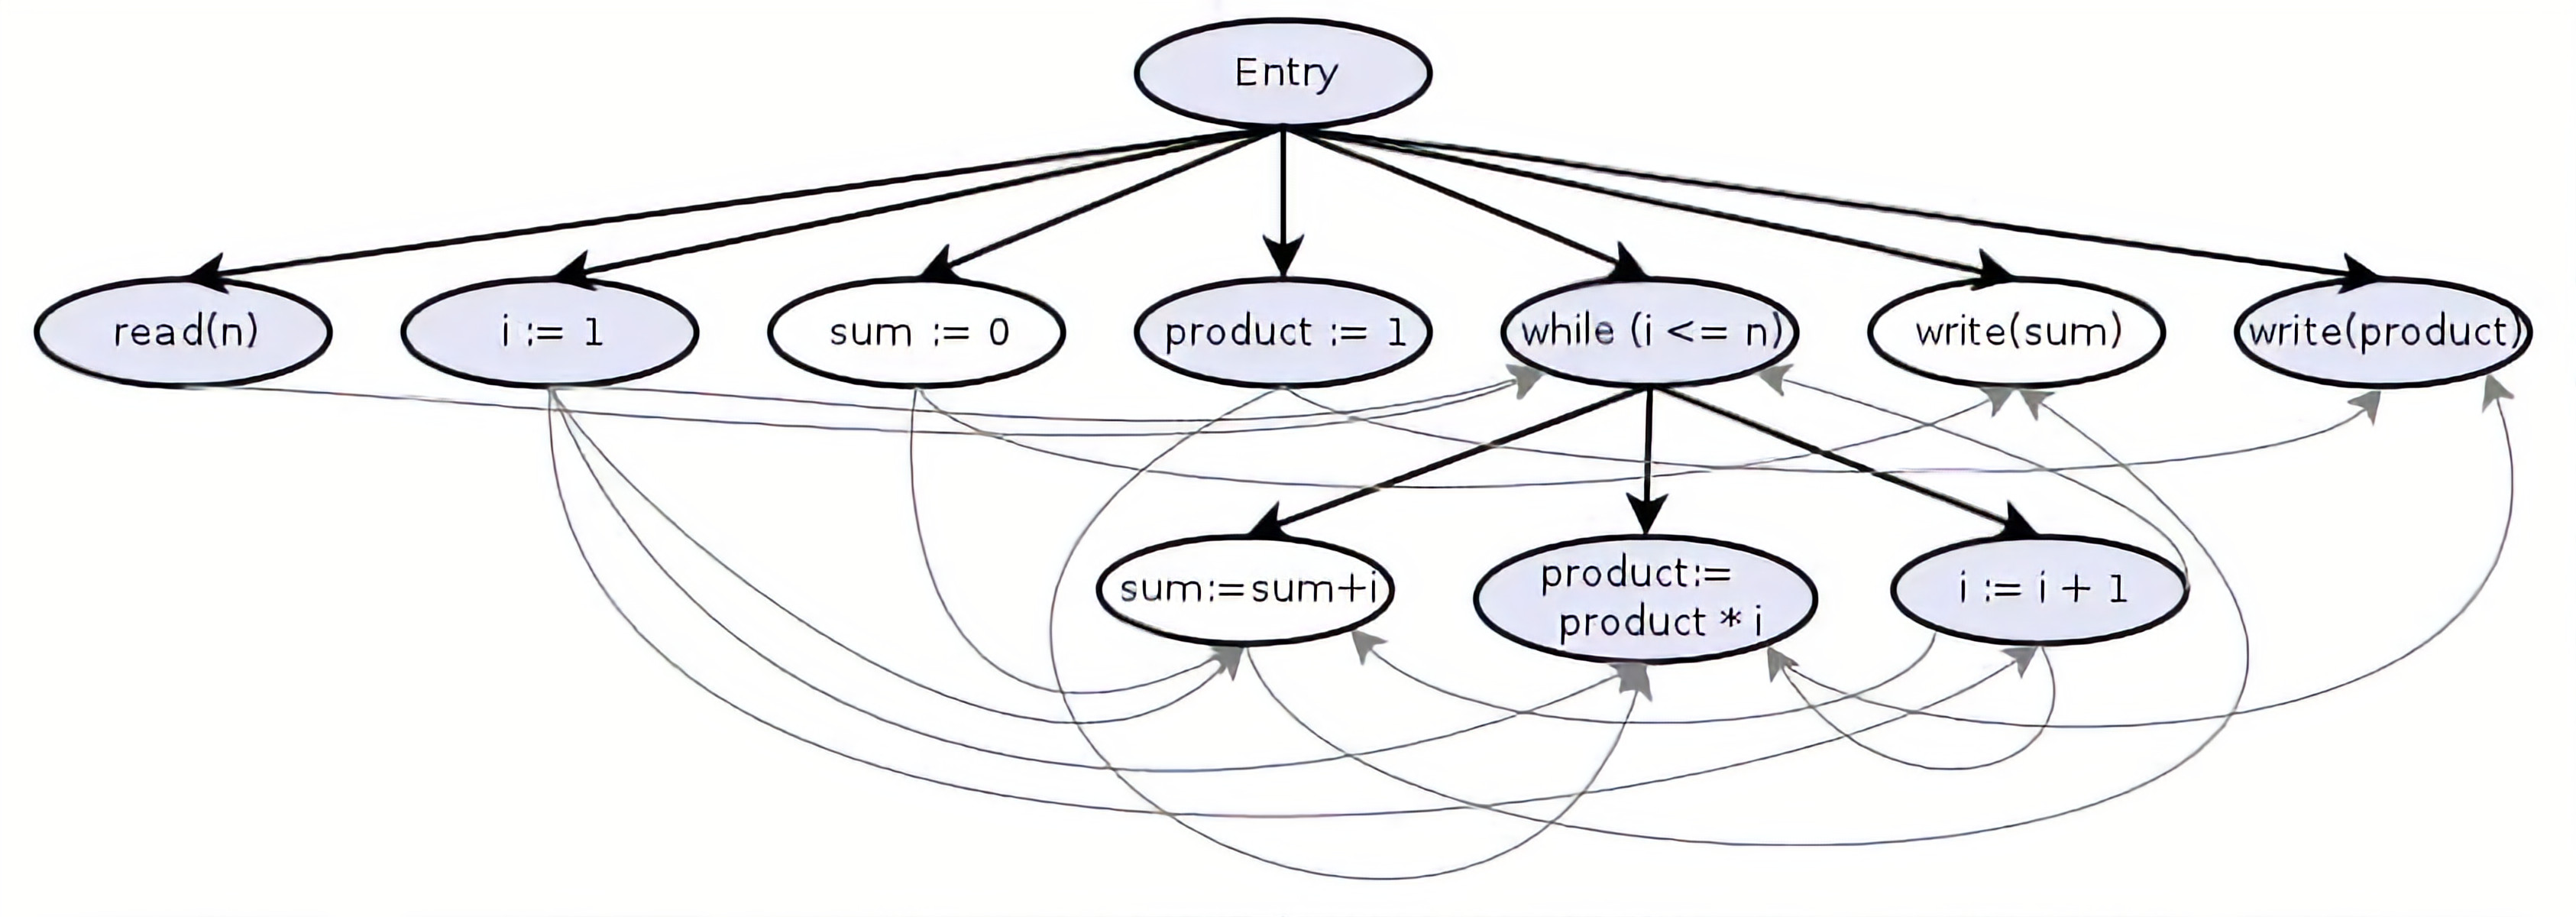
\includegraphics[width=0.75\textwidth]{pdg-example}
    \caption{Приклад графа програмних залежностей \cite{pdg-example}}
    \label{fig:pdg-example}
\end{figure} 
Дві частини програми вважаються ідентичними, якщо їх графи ізоморфні.
Головною перевагою є те, що цей граф не залежить від переставлення інструкцій, зміни назв функцій, тощо; не залежить від аспектів реалізації.
Недоліки методу:
\begin{itemize}
\item Дуже довгий час роботи, оскільки завдання пошуку ізоморфних підграфів є NP-повною, і може бути вирішена за поліноміальний час тільки для планарних графів, що не обов'язково виконається для графа програмних залежностей;
\item Такий метод не зможе знайти дублікати у коді, який не виконується у загальному випадку, оскільки у граф додаються лише виконані інструкції.
\end{itemize}
Приклад використання: \cite{Liu06}.
\subsubsection{Метод порівняння дерев}
У цьому методі використовуються абстрактні синтаксичні дерева (АСД). Згідно з \cite{wiki:ast}, абстрактне синтаксичне дерево -- позначене і орієнтоване дерево, в якому внутрішні вершини співставлені з відповідними операторами мови програмування, а листя з відповідними операндами.
\begin{figure}[h!]
    \centering
    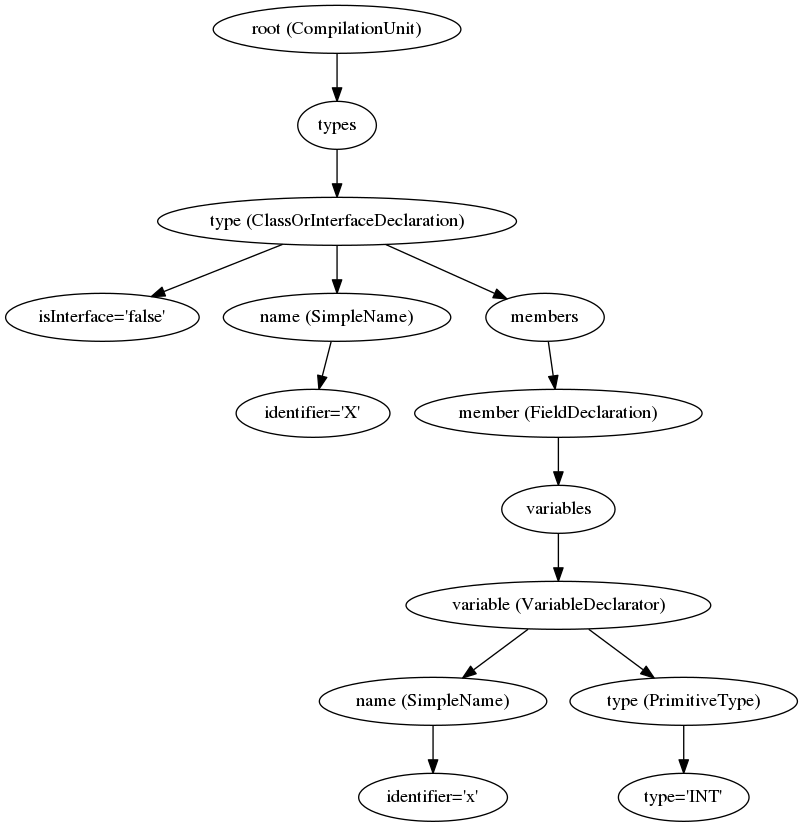
\includegraphics[width=0.5\textwidth]{ast-example}
    \caption{Приклад абстрактного синтаксичного дерева \cite{ast-example}}
    \label{fig:pdg-example}
\end{figure}\\
Щоб визначити, чи є частина коду копією іншої частини, знаходять відповідні їм піддерева, а далі ці піддерева порівнюються між собою. \\
Підходів до порівяння піддерев досить багато. Так, наприклад, у роботі \cite{Sager06} усі піддерева, що відповідають класам у початковому коді, порівнюються кожен з кожним за допомогою обчислення відстані між деревами. Автор відмічає, що цей метод є найточнішим порівняно з іншими, але має дуже довгий час роботи. Наприклад, код плагінів \verb|org.eclipse.compare-plug-in|, що складався зі 114 класів перевірявся на копії більше ніж годину. \\
У роботі \cite{Baxter98} теж стверджується, що алгоритм знахождення відстані між деревами має занадто велику складність обчислення, тому автором був запропонований інший підхід. Усі піддерева гешуються за допомогою вибраної <<поганої>> геш-функції та розподіляються у $B$ бакетів, де $B \approx N/10$. 
Далі кожне піддерево порівнюється лише з піддеревами з цього ж бакету за формулою: $$\textup{Схожість} = \frac{2*S}{2*S+L+R}.$$ $S$ -- кількість однакових вершин у обох піддеревах, $L$ -- кількість вершин, що присутні лише у першому піддереві, $R$ -- кількість вершин, що є тільки у другому піддереві. \\
Отже, головними перешкодами до використання цього методу є:
\begin{itemize} 
\item Великі час роботи та алгоритмічна складність; \cite{Ain19}
\item Досить низький відсоток знайдених копій через використання додаткових евристик. \cite{Dang15}
\end{itemize}
Далі буде запропоновано новий підхід, що значно зменшить час роботи, необхідний для знаходження копій, та, у той же час, збільшить ефективність їх знаходження.
\section{Новий алгоритм пошуку повторюваних частин}
Алгоритм складається із 4 кроків:
\begin{enumerate}
\item парсинг коду та перетворення його у абстрактне синтаксичне дерево;
\item визначення частин коду, які має сенс порівнювати;
\item знаходження повторюваних частин;
\item перетворення знайденого результату до конкретних елементів у коді.
\end{enumerate}
Далі опишемо детальніше кожен крок.
\subsection{Парсинг коду}
Компілятор практично будь-якої мови програмування на якомусь кроку перетворює код у абстрактне синтаксичне дерево. Для простоти, будемо працювати з кодом, написаним на мові програмування \verb|Java|. Щоб перетворити код у абстрактне синтаксичне дерево, використаємо \verb|JavaParser|. Алгоритм не складно змінити для підтримки будь-якої іншої мови програмування.
\subsection{Визначення частин коду, які підлягають порівнянню}
У загальному випадку, структура коду у об'єктно-оріентованих мовах программування виглядає таким чином: \\
\begin{figure}[h!]
\begin{lstlisting}[frame=none, xleftmargin=.3\textwidth]
import com.google.tools;
class X {
	int a=0;
	X(int a, int b)	{
		this.a = a;
	}
	void incrementAndPrint()	{
		a++;
	}
}
\end{lstlisting}
\caption{Приклад коду у об'єктно-орієнтованих мовах програмування}
\end{figure} \\
Можна визначити головні елементи практично кожної програми, а саме:
\begin{itemize}
\item підключення інших пакетів, бібліотек;
\item декларування класу та його елементи (поля);
\item декларування функцій та обчислення якогось результату.
\end{itemize}
Порівнянню і подальшому опрацюванню підлягають лише ті частини коду, які можна винести до іншої функції.
Цими елементами є тільки ствердження у функціях.\\
Пояснемо на прикладі: \\
\begin{figure}[h!]
\begin{lstlisting}[frame=none, xleftmargin=.3\textwidth]
import com.google.tools;
class X {
	int a=0;
	X(int a)	{
		[*this.a = a;*]
	}
	void incrementAndPrint()	{
		[*a++;
		print(a);*]
	}
}
\end{lstlisting}
\caption{Приклад коду}
\end{figure} \\
Курсивом виділені фрагменти коду, що будуть далі опрацьовані. \\
Визначимо вираз (<<expression>>) як найменшу неподільну операцію та параметр до цієї операції. \\ Будь яке велике обчислення можна розбити на вирази. \\
У операціях розгалуження вважатимемо виразами лише додаткові умови у них, але не самі операції. \\
Блок -- непорожня послідовність виразів, укладених між фігурними дужками та впорядкованих за порядком обходу алгоритма DFS у абстрактному синтаксичному дереві. \\
Алгоритм розбиває код на блоки таким чином, що вміст одного блоку не зустрічається у іншому. \\
В кожного виразу є свої координати: перша координата($x$) -- номер блоку, у якому є цей вираз, друга координата($y$) -- знаходження виразу у блоці.
\begin{figure}[h!]
\centering
\begin{minipage}{.4\textwidth}
\begin{lstlisting}[frame=none]
void func(){
	int x = 10;
	x = x+1;
	while (x>3){
		System.out.println(x*2);
		x--;
	}
}
\end{lstlisting}
\end{minipage}
\begin{minipage}{.5\textwidth}
\begin{lstlisting}[frame=none]
[int x = 10;, x = x + 1;, x > 3, System.out.println(x * 2);, x--;]
\end{lstlisting}
\end{minipage}
\caption{Приклад розбиття коду на вирази у блоці}
\end{figure} \\ \null \\
Порівнянню з іншою послідовністю підлягає будь-яка послідовність виразів, що йдуть поспіль, та знаходяться у одному блоці. \\
\subsection{Знаходження повторюваних частин}
У загальному випадку, у клонах є доволі багато ідентичних виразів. Для простоти будемо вважати, що клони починаються з ідентичного виразу. У майбутньому планується підтримка випадку, коли клони починаються не з ідентичного виразу. \\
Знаходження повторюваних частин працює наступним чином:
\begin{itemize}
\item для кожного виразу обчислити геш-функцію для кожного виразу;\\
У геш-функції враховуються усі типи кожного з вершин АСД, що лежать нижче, ніж відповідна вершина до цього виразу; типи буквальних виразів (наприклад, \verb|123.0f| це тип \verb|float|, \verb|"123"| -- тип \verb|String|).
\item{створити асоціативний масив, де ключем є геш, а значенням є список координат усіх виразів;}
\item{перетворити асоціативний масив на масив зі списків до кожного ключа;}
\item{відсортувати масив за зростанням наступної функції: $$f(list)=\max_{\forall expr \in list}{expr_{y}} $$ \\
Це потрібно для того, щоб потенційний відрізок не обмежувався іншим, вже відміченим як копію, відрізком.}
\item{для кожного списка координат з цього масива: 
\begin{enumerate}
\item{Знайти максимум функції: $$F(len)=(len-2*T-1)*goodGraphs-len-2$$
Де $len$ -- довжина відрізка виразів. При обчисленні функції створюється дерево структури відрізка виразів, де кожний вираз зустрічається один раз. \\
Один вираз є батьком (<<parent>>) іншого, якщо перший вираз є частиною операції розгалуження, і другий вираз знаходиться у тілі цієї операції. \\
В кожної вершини є свій надпис (<<label>>). Вважатимемо надписом кожної вершини тип відповідного виразу. \\
\begin{figure}[h]
    \centering
    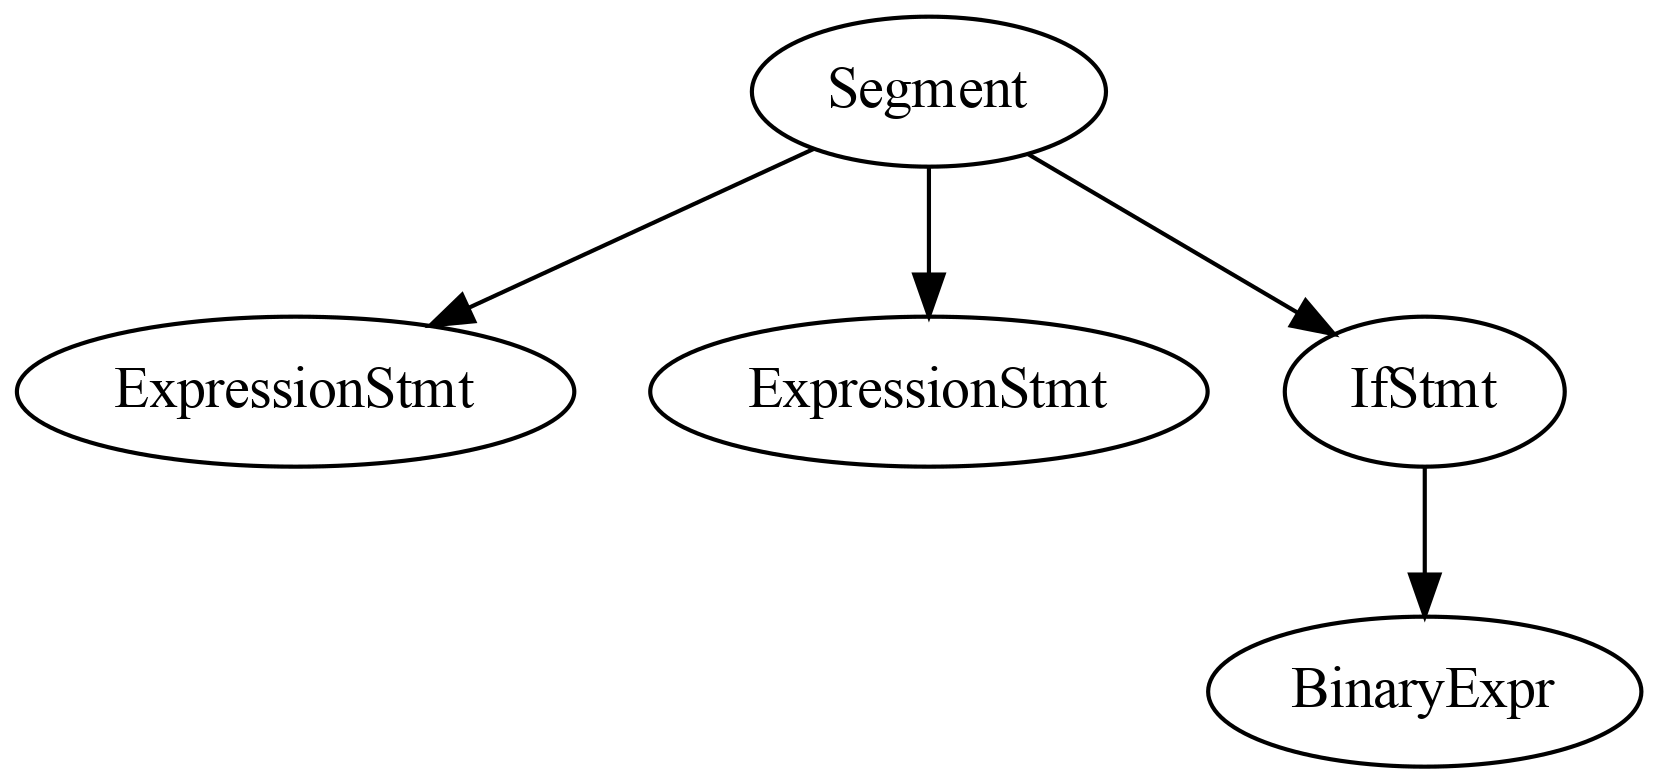
\includegraphics[width=0.75\textwidth]{function_graph_example}
    \caption{Приклад створюваного графу}
    \label{fig:}
\end{figure} \\
$goodGraphs$ -- кількість графів (окрім першого), для яких відстань зміни графа до першого є меншою за константу $T$\footnote{Відстань зміни графа обчислюється за допомогою алгоритму APTED. \cite{Pawlik15}\cite{Pawlik16}}. \\
Відстань зміни графа вимірюється за 3 параметрами: 
\begin{itemize}
\item вартість видалення вершини (дорівнює $0.5$);
\item вартість зміни <<надпису>> вершини (дорівнює $1$);
\item вартість вставки вершини (дорівнює $0.5$).
\end{itemize}
Для кращого знаходження дублікатів \RNum{3} типу, вартості видалення і вставки зменшені, 
тоді вартість переставлення виразу буде такою ж, як і вартість зміни <<надпису>>.\\
Слід зазначити, що $$D(F)=[3, maxPotentialLen] \backslash \forall len: $$
$$\exists piece, piece_y \geq start_y+len, piece \in varusages, $$
$$\exists decl, start_{y} \leq decl_{y} < start_{y}+len, $$
$$decl \in declarations, decl_{var}=piece_{var};$$
$$maxPotentialLen = min(exprCount, y_{nearest})-start_y,$$ де:
\begin{itemize} 
\item $3$ -- константа, обрана емпірічно, щоб відрізки меншої довжини не вважалися клонами, бо вони не мають сенсу для програміста.
\item $maxPotentialLen$ -- максимально можлива довжина відрізка;
\item $start$ -- почтаковий вираз відрізка;
\item $varusages$ -- множина усіх використань змінних у цьому відрізку;
\item $declarations$ -- множина усіх декларацій змінних у цьому відрізку;
\item $decl_{var}$, $piece_{var}$ -- імена відповідних змінних;
\item $exprCount$ -- кількість виразів у блоці;
\item $y_{nearest}$ -- y-координата найближчого виразу-клона.
\end{itemize}
Додаткова умова додана, щоб не було таких випадків, коли декларація використованої змінної вже відсутня.
$F(len)$ -- приблизна кількість рядків у коді, що будуть зекономлені.
$$F(len) = len*goodGraphs-goodGraphs-2*T*goodGraphs-len-2,$$ 
де:
\begin{itemize}
\item $len*goodGraphs$ -- приблизна початкова кількість рядків коду;
\item $goodGraphs$ -- кількість потрібних викликів нової функції, кожен виклик зазвичай займає 1 рядок;
\item $2*T*goodGraphs$ -- приблизна кількість рядків коду, потрібного для врахування усіх відмінностей між послідовностями виразів;
\item $len$ -- приблизна кількість рядків коду, що є повністю ідентичним між усіма послідовностями;
\item $2$ -- кількість рядків, необхідна щоб записати функцію у коді.
\end{itemize}
$$F(len) = len*goodGraphs-goodGraphs-2*T*goodGraphs-len-2$$
$$F(len) = (len-1)*goodGraphs-2*T*goodGraphs-len-2$$
$$F(len) = (len-2*T-1)*goodGraphs-len-2$$
}
\item Якщо кількість відрізків більша за $1$ і $F(len)>0$, то усі вирази у відрізку відмітити як вирази-клони.
$F(len)$ повинно бути більше ніж 0, бо у інакшому випадку у сгенерованому коді буде більше рядків, а це не має сенсу.
\end{enumerate}
}
\end{itemize}
\subsection{Перетворення на послідовність фрагментів у коді}
Попереднім кроком були знайдені усі вирази-клони, але їх ще потрібно перетворити у послідовність фрагментів, бо самі по собі вирази показують лише уривки з початкового коду.   
\begin{figure}[h!]
\centering
\begin{minipage}{.5\textwidth}
\begin{lstlisting}[frame=none]
[xx == 466.0f,xx == 143.0f,xx == 466.0f,xx++;,xx == 143.0f,xx++;]
\end{lstlisting}
\end{minipage}
\begin{minipage}{.4\textwidth}
\begin{lstlisting}[frame=none]
if (xx==466.0f || xx==143.0f) {
  if (xx==466.0f)
		xx++;
	else if (xx==143.0f)
		xx++;
}	
\end{lstlisting}
\end{minipage}
\caption{Приклад послідовності виразів-клонів та відповідна їм частина коду}
\end{figure} \\
Зробимо перетворення наступним чином: оберемо усі вершини у абстрактному синтаксичному дереві (АСД), для яких
$$\exists piece, LCA(son, piece_{ast}) = son,$$
де:
\begin{itemize}
\item $son$ -- син закріпленої за блоком вершини у АСД, 
\item $piece$ -- вираз, 
\item $piece_{ast}$ -- відповідна виразу вершина у АСД.
\end{itemize}
Таким чином, для послідовності виразів-клонів закріплені вершини у абстрактному синтаксичному дереві.
У подальшому називатимемо ці вершини інструкціями.
\subsection{Використання алгоритму для видалення клонів}
Для видалення списка повторюваних частин коду об'єднаємо їх у функцію. \\
Зробимо це наступним алгоритмом: 
\begin{enumerate}
\item Кожна повторювана частина коду являє собою список інструкцій. \\
Тілом функції буде найбільша спільна підпослідовність цих списків.
\item Виконання кожної іншої інструкції, що не війшла до найбільшої спільної підпослідовності, обернемо у оператор \verb|if|.
Умовою цього оператору стане параметр функції типу \verb|boolean|.
\item Додати до усіх використаних змінних, полів, викликів функцій з іншої частини коду назву класу.
\item Усі буквальні вирази, що є у найбільшій спільній підпослідовності, та не є однаковими для усіх відповідних інструкцій, замінимо на параметр функції. Тип параметру може бути визначений за допомогою бібліотеки \verb|JavaParser|.
\item Для кожної повторюваної частини замінити першу інструкцію у списку на виклик нової функції, інші інструкції видалити.
\item Нову функцію записати у файл \verb|Copied.java|.
\end{enumerate}
\newpage
\begin{figure}[h!]
\centering
\begin{minipage}{.45\textwidth}
\begin{lstlisting}[frame=none]
static final double PI = 3.1415;
static void veryImportantFunction()
{
	double xx = Math.cos(PI/2)-Math.sin(PI/2);
	double yy = Math.sin(PI/2)+Math.cos(PI/2);
	if (xx==456.0f || xx==123.0f){
		if (xx==456.0f)
			xx++;
		else if (xx==123.0f)
			xx++;
	}
	xx*=2;
	yy*=2;
	System.out.println(xx+" "+yy);
}
\end{lstlisting}
\end{minipage}
\begin{minipage}{.45\textwidth}
\begin{lstlisting}[frame=none]
static final double PI = 3.1415;
static void superComputing()
{
	double aa = Math.cos(PI/2)-Math.sin(PI/2);
	double bb = Math.sin(PI/2)+Math.cos(PI/2);
	if (aa==345.0f || aa==0f){
		if (aa==345.0f)
			aa++;
		else if (aa==0.0f)
			aa++;
	}
	aa*=2;
	bb*=2;
	System.out.println(aa+" "+bb);
}
\end{lstlisting}
\end{minipage}
\caption{Приклад коду до виконання алгоритмів}
\end{figure}

\begin{figure}[h!]
\centering
\begin{minipage}{.4\textwidth}
\begin{lstlisting}[frame=none]
static final double PI = 3.1415;
static void veryImportantFunction() {
  Copied.
    veryImportantFunction(456.0f, 123.0f, 456.0f, 123.0f);
}
static void superComputing() {
  Copied.
    veryImportantFunction(345.0f, 0f, 345.0f, 0.0f);
}
\end{lstlisting}
\end{minipage}
\begin{minipage}{.55\textwidth}
\begin{lstlisting}[frame=none]
static final double PI = 3.1415;
static void veryImportantFunction(Double literalXx, Double literalXx2, Double literalXx3, Double literalXx4) {
  double xx = Math.cos(Main.PI / 2) - Math.sin(Main.PI / 2);
  double yy = Math.sin(Main.PI / 2) + Math.cos(Main.PI / 2);
  if (xx == literalXx || xx == literalXx2) {
    if (xx == literalXx3)
      xx++;
    else if (xx == literalXx4)
      xx++;
  }
  xx *= 2;
  yy *= 2;
	System.out.println(xx+" "+yy);
}
\end{lstlisting}
\end{minipage}
\caption{Приклад роботи обох алгоритмів: знаходження та видалення клонів}
\end{figure} 
\section{Порівняння з іншими методами}
Порівняємо запропонований алгоритм з іншими методами. \\
Існують різні способи порівняння методів пошуку дублікатів у коді, доволі часто використованим способом є бенчмарк \cite{Bellon07}. \\
Проте, у роботі \cite{Vislavski18} зазначається, що цей бенчмарк може бути необ'єктивним, оскільки перевірка того, чи дійсно 2 частини коду є клонами виконується людиною, тому у використованих при розробці бенчмарка інструментів з'являється додаткова перевага. Також відмічається, що у новому бенчмарку <<BigCloneEval>> \cite{Svajlenko14} ця проблема нівельована, тому будемо використовувати саме його. \\
Зазвичай порівняння виконується за 2 основними параметрами: 
\begin{itemize}
\item Точність (<<precision>>). Інструмент повинен бути детектувати якомога менше хибно-позитивних клонів. \\ Точність обчислюється як відношення правильно знайдених пар клонів до усіх знайдених інструментом пар клонів.
\item Відклик (<<recall>>). Інструмент має коректно знаходити більшість пар клонів серед можливих (тобто відмічених людиною). \\ Відклик обчислюється як відношення кількості коректно знайдених пар клонів до кількості відмічених людиною пар клонів.
\item Час роботи інструменту.
\end{itemize}
Для порівняння з новим алгоритмом обрані наступні програми:
\begin{itemize}
\item \verb|CCFinderX|;
\item \verb|PMD|;
\item \verb|CloneDR|.
\end{itemize}
Ці програми є реалізаціями різних методів, описаних у розділі \ref{sec:characteristics}.
Виконаємо порівняння на наступному обладнанні: 
\begin{itemize}
\item процесор -- \verb|Intel Core i5-8250U|, 1.60Ггц
\item оперативна пам'ять -- 8 Гб;
\item операційна система -- \verb|Windows 10|.
\end{itemize} 
Отримані наступні результати: \\
\begin{table}[ht]
\centering
 \begin{tabular}{| c | c | c |} 
 \hline
 Назва інструменту & Точність & Відклик \\ [0.5ex] 
 \hline
 \verb|CCFinderX| & 0.57 & 0.5 \\ 
 \hline
 \verb|PMD| & 0.48 & 0.58 \\
 \hline
 \verb|CloneDR| & 0.82 & 0.47 \\
 \hline
 Новий алгоритм & 0.76 & 0.53 \\ [1ex]
 \hline
\end{tabular} 
\caption{Порівняння інструментів знаходження клонів}
\end{table} \\
Як бачимо, новий алгоритм є значно точнішим, ніж інструменти \verb|CCFinderX|, \verb|PMD| менш точним ніж \verb|CloneDR|, проте в цього інструменту відклик є меншим. \\
Відклик нового алгоритму є більшим, ніж у всіх програм, окрім \verb|PMD|, в якого точність є значно меншою. \\
Порівняємо час роботи алгоритму із іншими програмами на початковому коді наступних проектів:
\begin{itemize}
\item DnsJava ($\sim$40000 рядків коду);
\item JFreeChart ($\sim$300000 рядків);
\item Tomcat ($\sim$600000 рядків);
\item OpenOffice ($\sim$800000 рядків).
\end{itemize}
Отримані результати наведені у таблиці.
\begin{table}[h]
\centering
 \begin{tabular}{| c | c | c | c | c |} 
 \hline
 \bigcell{c}{\\ Час обробки проекту (с), \\ Назва інструменту \\ {}} & {\verb|DnsJava|} & \verb|JFreeChart| & \verb|Tomcat| & \verb|OpenOffice|  \\ [0.5ex] 
 \hline
 \verb|CCFinderX| & 12 & 64 & 195 & 289 \\ 
 \hline
 \verb|PMD| & 1 & 3 & 5 & 15 \\
 \hline
 \verb|CloneDR| & 18 & 270 & 1378 & 3249 \\
 \hline
 Новий алгоритм & 5 & 19 & 59 & 97 \\ [1ex]
 \hline
\end{tabular} 
\caption{Потрібний інструментам час для обробки різних проектів}
\end{table} \\
Можна побачити, що новий алгоритм є значно швидшим, ніж \verb|CCFinderX| та \verb|CloneDR|, але повільнишим, ніж \verb|PMD|. \\
Він є оптимальним варіантом за обраними показниками.
\section{Висновки}
Виділені 4 головних типи повторюваних частин:
\begin{itemize}
\item \RNum{1} тип -- повна копія практично з відсутніми модифікаціями;
\item \RNum{2} тип -- змінюються лише назви змінних, функцій, класів;
\item \RNum{3} тип -- копія із доданими, зміненими, або видаленими інструкціями, зміненими назвами об'єктів;
\item \RNum{4} тип -- копія, що значно відрізняється синтаксично, але робить ідентичні обчислювання.
\end{itemize}
Були проаналізовані наступні методи знаходження повторюваних частин у початковому коді програмного забезпечення:
\begin{itemize}
\item пошук збігу рядків початкового коду;
\item використання токенів;
\item метод порівняння функцій;
\item застосування графа програмних залежностей;
\item метод порівняння дерев.
\end{itemize} 
Виявлені основні переваги і недоліки кожного з методів. \\ 
Створений новий алгоритм, який усуває недоліки методу порівняння дерев, а саме:
\begin{itemize}
\item Надто великі час роботи та алгоритмічна складність;
\item Досить низький коефіцієнт відклику через використання додаткових евристик.
\end{itemize}
Зроблено порівняння між новим алгоритмом та існуючими методами за 3 основними показниками: точністю, відкликом та часом роботи. \\
Продемонстровано, що новий метод є оптимальним: має задовільні показники точності та відклику (0.76 та 0.53 відповідно); проект із $\sim$800000 рядків коду оброблюється менш, ніж за 2 хвилини.
\printbibliography[title={список використаних джерел}]
\end{document}
